%! Author = Omar Iskandarani
%! Title = Vortex-String Theory as an Emergent Relativistic Effective Field Theory with Preferred Foliation
%! Date = Aug 22, 2025
%! Affiliation = Independent Researcher, Groningen, The Netherlands
%! License = © 2025 Omar Iskandarani. All rights reserved. This manuscript is made available for academic reading and citation only. No republication, redistribution, or derivative works are permitted without explicit written permission from the author. Contact: info@omariskandarani.com
%! ORCID = 0009-0006-1686-3961
%! DOI = 10.5281/zenodo.16923312


\newcommand{\papertitle}{Vortex-String Theory as an Emergent Relativistic Effective Field Theory with Preferred Foliation}
\newcommand{\paperdoi}{10.5281/zenodo.16923312}

\documentclass[12pt]{article}
% vamstyle.sty
\NeedsTeXFormat{LaTeX2e}
\ProvidesPackage{vamstyle}[2025/06/13 VAM unified style]

\newif\ifvamdraft
% Uncomment the next line to enable draft mode:
% \vamdrafttrue

\ifvamdraft
  \RequirePackage{showframe} % shows margins for debugging
\fi

\RequirePackage{ifthen}
\newboolean{vamstyleloaded}
\ifthenelse{\boolean{vamstyleloaded}}{}{\setboolean{vamstyleloaded}{true}

\RequirePackage[a4paper, margin=2cm]{geometry}

% -- Fonts and Language --
\RequirePackage[T1]{fontenc}
\RequirePackage[utf8]{inputenc}
\RequirePackage[english]{babel}
\RequirePackage{mathpazo}           % or newtxtext/newtxmath
\RequirePackage[scaled=0.95]{inconsolata}
\RequirePackage{helvet}

% Math and Physics
\RequirePackage{amsmath, amssymb, mathrsfs, physics}
\RequirePackage{siunitx}
\sisetup{per-mode=symbol}

% -- Tables and Figures --
\RequirePackage{graphicx, float, booktabs}
\RequirePackage{array, tabularx, multirow, makecell}
\RequirePackage[font=footnotesize, labelfont=bf]{caption}
\RequirePackage{subcaption}
% Safe wide table environment (auto-fit to text width)
\newcolumntype{Y}{>{\centering\arraybackslash}X} % Like 'X' but centered
\newenvironment{tighttable}[1][] % optional argument = caption
  {\begin{table}[H]\centering\renewcommand{\arraystretch}{1.3}
   \begin{tabularx}{\textwidth}{#1}}
  {\end{tabularx}\end{table}}
% Force fit large tables without changing layout
\RequirePackage{etoolbox}
\newcommand{\fitbox}[2][\linewidth]{\makebox[#1]{\resizebox{#1}{!}{#2}}}

% Graphics and Diagrams
\RequirePackage{tikz}
\usetikzlibrary{arrows.meta, positioning}
\RequirePackage{pgfplots}
\pgfplotsset{compat=1.18}
\RequirePackage{xcolor}

% -- Code Listings --
\RequirePackage{listings}
\lstset{basicstyle=\ttfamily\footnotesize, breaklines=true}

% TOC Customization
\RequirePackage{tocloft}
\setcounter{tocdepth}{2}
\renewcommand{\cftsecfont}{\bfseries}
\renewcommand{\cftsubsecfont}{\itshape}
\renewcommand{\cftsecleader}{\cftdotfill{.}}
\renewcommand{\contentsname}{\centering \Huge\textbf{Contents}}

% Section Fonts
\RequirePackage{sectsty}
\sectionfont{\Large\bfseries\sffamily}
\subsectionfont{\large\bfseries\sffamily}

% Bibliography
\RequirePackage[numbers]{natbib}

% PDF Links and Metadata
\RequirePackage{hyperref}
\hypersetup{
    colorlinks=true,
    linkcolor=blue,
    citecolor=blue,
    urlcolor=blue,
    pdftitle={The Vortex Æther Model},
    pdfauthor={Omar Iskandarani},
    pdfkeywords={vorticity, gravity, æther, fluid dynamics, time dilation, VAM}
}

\urlstyle{same}
\RequirePackage{bookmark}

% Line Breaking and Style
\RequirePackage[none]{hyphenat}
\sloppy


\usepackage[most]{tcolorbox}
\usepackage{graphicx}
\usepackage{titling}

\pretitle{\begin{center}\LARGE\bfseries}
\posttitle{\par\end{center}\vskip 0.5em}
\preauthor{\begin{center}\large}
\postauthor{\end{center}}
\predate{\begin{center}\small}
\postdate{\end{center}}


\endinput
}
% -- End of vamstyle.sty --
% vamappendixsetup.sty

\newcommand{\titlepageOpen}{
  \begin{titlepage}
    \thispagestyle{empty}
    \centering
    \vspace*{2cm}
    {\Huge\bfseries \appendixtitle \par}
    \vspace{1cm}
    {\Large\itshape \appendixauthor \par}
    \vspace{0.5cm}
    {\small \appendixaffil \par}
    ORCID: \href{https://orcid.org/\appendixorcid}{\appendixorcid} \\
    DOI: \href{https://doi.org/\appendixdoi}{\appendixdoi} \\
    \vspace{0.5cm}
    {\large \today \par}
    \vspace{1cm}
}

\newcommand{\titlepageClose}{
  \vfill
  \end{titlepage}
}



%========================================================================================
%   PACKAGES AND DOCUMENT CONFIGURATION
%========================================================================================

\usepackage[margin=1in]{geometry}
\usepackage{amsmath, amssymb}
\usepackage{graphicx}
\usepackage{hyperref}
\usepackage{authblk}
\usepackage{abstract}
\usepackage{fancyhdr}
\usepackage[backend=biber, style=numeric-comp, sorting=none]{biblatex}
\usepackage{filecontents}

%========================================================================================
%   BIBLIOGRAPHY DATA (CLEANED)
%========================================================================================

\begin{filecontents}{vst_references.bib}
    @article{Kelvin1867,
    author  = {Thomson, William (Lord Kelvin)},
    title   = {On Vortex Atoms},
    journal = {Philosophical Magazine},
    volume  = {34},
    pages   = {15--24},
    year    = {1867}
    }
    @article{Nielsen1973,
    author  = {Nielsen, H. B. and Olesen, P.},
    title   = {Vortex-line models for dual strings},
    journal = {Nuclear Physics B},
    volume  = {61},
    pages   = {45--61},
    year    = {1973}
    }
    @article{Faddeev1997,
    author  = {Faddeev, L. D. and Niemi, A. J.},
    title   = {Stable knot-like structures in classical field theory},
    journal = {Nature},
    volume  = {387},
    pages   = {58--61},
    year    = {1997}
    }
    @book{Arnold1998,
    author    = {Arnold, V. I. and Khesin, B. A.},
    title     = {Topological Methods in Hydrodynamics},
    publisher = {Springer},
    year      = {1998},
    series    = {Applied Mathematical Sciences},
    volume    = {125}
    }
    @article{Moffatt1969,
    author  = {Moffatt, H. K.},
    title   = {The degree of knottedness of tangled vortex lines},
    journal = {Journal of Fluid Mechanics},
    volume  = {35},
    number  = {1},
    pages   = {117--129},
    year    = {1969}
    }
    @book{Volovik2003,
    author    = {Volovik, G. E.},
    title     = {The Universe in a Helium Droplet},
    publisher = {Clarendon Press},
    year      = {2003},
    series    = {International Series of Monographs on Physics}
    }
    @article{Kleckner2013,
    author  = {Kleckner, Dustin and Irvine, William T. M.},
    title   = {Creation and dynamics of knotted vortices},
    journal = {Nature Physics},
    volume  = {9},
    pages   = {253--258},
    year    = {2013}
    }
    @article{Madelung1927,
    author  = {Madelung, E.},
    title   = {Quantentheorie in hydrodynamischer Form},
    journal = {Zeitschrift f{"u}r Physik},
    volume  = {40},
    pages   = {322--326},
    year    = {1927}
    }
    @article{BilsonThompson2007,
    author  = {Bilson-Thompson, Sundance O.},
    title   = {A topological model of composite preons},
    journal = {Foundations of Physics},
    volume  = {37},
    number  = {1},
    pages   = {69--89},
    year    = {2007}
    }
    @article{Barcelo2011,
    author  = {Barcel{\'o}, Carlos and Liberati, Stefano and Visser, Matt},
    title   = {Analogue Gravity},
    journal = {Living Reviews in Relativity},
    volume  = {14},
    number  = {3},
    year    = {2011}
    }
    @article{Podkletnov1992,
    author  = {Podkletnov, Eugene and Nieminen, R.},
    title   = {A possibility of gravitational force shielding by bulk YBa2Cu3O7−x superconductor},
    journal = {Physica C: Superconductivity},
    volume  = {203},
    pages   = {441--444},
    year    = {1992}
    }
    @article{Tajmar2006,
    author  = {Tajmar, M. and Plesescu, F. and Seifert, B. and Marhold, K.},
    title   = {Experimental Detection of the Gravitomagnetic London Moment},
    journal = {AIP Conference Proceedings},
    volume  = {880},
    number  = {1},
    pages   = {1071--1082},
    year    = {2006}
    }
    @article{cahill2005,
    author  = {Cahill, Reginald T.},
    title   = {Dynamical 3-Space: A Review},
    journal = {Progress in Physics},
    volume  = {3},
    pages   = {27--34},
    year    = {2005}
    }
    @book{Kauffman1991,
    author    = {Kauffman, Louis H.},
    title     = {Knots and Physics},
    publisher = {World Scientific},
    year      = {1991}
    }
    @book{Stasiak2009,
    editor    = {Stasiak, Andrzej and Katritch, Vasily and Kauffman, Louis H.},
    title     = {Ideal Knots},
    publisher = {World Scientific},
    year      = {2009}
    }
    @article{Moffatt1990,
    author  = {Moffatt, H. K.},
    title   = {The energy spectrum of knots and links},
    journal = {Nature},
    volume  = {347},
    pages   = {367--369},
    year    = {1990}
    }
    @book{NISTDLMF,
    author    = {{NIST Digital Library of Mathematical Functions}},
    title     = {NIST Digital Library of Mathematical Functions},
    publisher = {Release 1.1.9 of 2023-03-15},
    note      = {\url{https://dlmf.nist.gov/}}
    }
\end{filecontents}



%========================================================================================
%   TITLE PAGE
%========================================================================================

\begin{document}

    % === Title page ===
    \titlepageOpen


%========================================================================================
%   DOCUMENT START
%========================================================================================


    \renewcommand{\headrulewidth}{0pt}

    \begin{abstract}
        We recast a vortex--string description of matter and interactions into journal-standard effective field theory language. The underlying medium is a condensed vacuum endowed with a preferred foliation encoded by a clock field $T(x)$. Low-energy excitations appear relativistic in the subspace orthogonal to $\nabla_\mu T$. Stable knotted vortex strings in this medium furnish the particle spectrum, with their rest energies giving fermion masses, while coarse-grained vorticity yields an emergent non-Abelian \emph{swirl connection}. The action combines a two-form $B_{\mu\nu}$ with $\mathcal{H}=dB$, a Yang--Mills sector for the swirl connection, and covariant constraints enforcing a unit timelike vector $u_\mu\!\propto\!\partial_\mu T$. A genuinely topological $\mathcal{W}\tilde{\mathcal{W}}$ term enforces helicity quantization and knot stability. We present a topological mass functional whose parameters are fixed by condensate scales and knot invariants and outline a calibration strategy against the electron, proton, and neutron. The framework aligns with analogue-gravity and topological-soliton programs \cite{Barcelo2011,Faddeev1997,Moffatt1969,Arnold1998,Volovik2003,Kleckner2013} while dispensing with free Yukawa couplings.
    \end{abstract}
    \titlepageClose

    \newpage

%========================================================================================
%   INTRODUCTION
%========================================================================================
    \section{Introduction}

    The Standard Model and General Relativity capture a wide range of phenomena but rely on disparate principles and mathematical structures. An alternative is that both matter and interactions emerge from a structured, condensed vacuum, continuing a lineage from Kelvin's vortex atoms \cite{Kelvin1867}, to hydrodynamic formulations of quantum theory \cite{Madelung1927}, to modern topological solitons and analogue gravity \cite{Faddeev1997,Arnold1998,Barcelo2011,Volovik2003,Kleckner2013}. We develop an effective field theory (EFT) in which a preferred foliation (a ``clock'' field) endows the vacuum with order. In this medium, stable knotted vortex strings constitute the particle spectrum; their interactions arise from an emergent non-Abelian gauge structure built from coarse-grained vorticity.

    Our aim is to present the ontology and equations in a form compatible with conventional EFT practice while maintaining the core claim: fermion masses are non-perturbative soliton energies rather than parameters introduced via fundamental Higgs--Yukawa couplings. Where possible, we emphasize covariant formulations and truly topological densities, avoiding mixed nonrelativistic--relativistic constructs.

%========================================================================================
%   FIELDS AND GEOMETRY
%========================================================================================
    \section{Foundational Fields and Geometry}

    The EFT is built from the following fields and geometric structures on a spacetime with metric $g_{\mu\nu}$ (signature $-\!+\!+\!+$):
    \begin{itemize}
        \item \textbf{Clock Field $T(x)$ and Preferred Foliation:} We define the unit timelike 4-vector field of the condensate as
        \begin{equation}
            u_{\mu} \equiv \frac{\partial_{\mu}T}{\sqrt{-\partial_{\alpha}T \partial^{\alpha}T}},
        \end{equation}
        which satisfies $u^\mu u_\mu = -1$ under a $(-+++)$ metric signature. This definition ensures $u_\mu$ is always real and properly normalized, provided $T$ is a smooth scalar field with timelike gradient.


        \item \textbf{Condensate Modulus $\Phi$:} A real scalar describing amplitude fluctuations of the ordered vacuum. It is \emph{not} a Standard Model Higgs; its role is to set medium scales (e.g., stiffness, characteristic speeds).

        \item \textbf{Two-Form Potential $B_{\mu\nu}$ and Three-Form Field Strength $\mathcal{H}$:}
        \begin{equation}
            \mathcal{H}_{\mu\nu\rho} \equiv \partial_{[\mu} B_{\nu\rho]}\,.
        \end{equation}
        Vortex strings are electrically coupled to $B$; their topological charge is measured by fluxes of $\mathcal{H}$.

        \item \textbf{Emergent Swirl Connection $\mathcal{A}_\mu^a$:} An effective non-Abelian gauge potential capturing coarse-grained vorticity modes. The corresponding field strength is
        \begin{equation}
            \mathcal{W}_{\mu\nu}^a = \partial_\mu \mathcal{A}_\nu^a - \partial_\nu \mathcal{A}_\mu^a + g_{\!sw}\, f^{abc}\,\mathcal{A}_\mu^b\,\mathcal{A}_\nu^c\,.
        \end{equation}

        \item \textbf{Knot Fermion Fields $\Psi_K$:} Relativistic spinors corresponding to stable knotted vortex strings labeled by a topological class $K$ (e.g., torus knots), with masses given by their soliton energies $m_K^{(\mathrm{sol})}$.
    \end{itemize}

%========================================================================================
%   EFFECTIVE ACTION (CONSISTENT, COVARIANT)
%========================================================================================
    \section{Effective Action}

    A minimal, consistent Lagrangian density that implements the above ingredients is
    \begin{align}
        \mathcal{L} =\;& -\frac{\kappa_\omega}{4}\, \mathcal{W}^a_{\mu\nu}\,\mathcal{W}^{a\mu\nu}
        + \frac{1}{2} (\nabla_\mu \Phi)(\nabla^\mu \Phi) - V(\Phi)
        + \frac{\kappa_B}{12}\, \mathcal{H}_{\mu\nu\rho}\,\mathcal{H}^{\mu\nu\rho}
        + \frac{\theta}{4}\, \mathcal{W}^a_{\mu\nu}\,\tilde{\mathcal{W}}^{a\mu\nu} \\
        &+ \lambda_1\,(u_\mu u^\mu + 1) + \lambda_2\, \nabla_\mu u^\mu
        + \sum_K \overline{\Psi}_K\big(i\gamma^\mu D_\mu - m_K^{(\mathrm{sol})}\big)\Psi_K\,,
        \label{eq:EFT}
    \end{align}
    with $\tilde{\mathcal{W}}^{a\mu\nu} \equiv \tfrac{1}{2} \epsilon^{\mu\nu\rho\sigma} \mathcal{W}^a_{\rho\sigma}$ and $D_\mu = \partial_\mu + i g_{\!sw}\,\mathcal{A}_\mu^a T^a$. The Lagrange multipliers $\lambda_{1,2}$ enforce a unit timelike $u^\mu$ and covariant incompressibility $\nabla_\mu u^\mu=0$ (if desired). The $\mathcal{W}\tilde{\mathcal{W}}$ term is topological and encodes helicity/knot-charge conservation \cite{Moffatt1969,Arnold1998}.

    The swirl gauge field \( \mathcal{A}_\mu^a \) emerges as a mesoscopic coarse-graining of vortex structure; see Appendix~\ref{app:swirl-connection} for a derivation sketch.

    \paragraph{Spinor Fields and Emergent Fermions.}
    We include a Dirac spinor term in the Lagrangian to describe the dynamics of the knotted excitations:
    \begin{equation}
        \mathcal{L}_\text{spinor} = \bar{\Psi}_K \left( i\gamma^\mu D_\mu - m_K \right) \Psi_K,
    \end{equation}
    where $\Psi_K$ is associated with a specific topological class of vortex excitation.

    This term is not fundamental, but emerges as an effective description of the low-energy collective modes of the underlying fluid-vortex structure. Analogous to how phonons and rotons appear in superfluid helium, or how quasiparticles emerge in topological condensed matter systems, these spinors represent stabilized, quantized vortex structures with internal orientation degrees of freedom, see Fig.~\ref{fig:emergent-spinors} for a schematic overview.

    Future work should aim to derive the Dirac-like dynamics from first principles by coarse-graining the vortex field equations, possibly following the approach of analogue gravity and superfluid analogs \cite{Barcelo2005,Volovik2009,CarterLanglois1995}.

    The spinors $\Psi_K$ transform under the swirl gauge group $G_{sw}$, representing internal symmetry structures of the knotted vortex states. The covariant derivative $D_\mu = \partial_\mu + i g_{sw} \mathcal{A}_\mu^a T^a$ reflects their interaction with coarse-grained vorticity modes.

    \paragraph{Remarks.} (i) We do not introduce fundamental Yukawa couplings; fermion masses enter only via soliton energies. (ii) Gauge-boson mass generation, if present, arises from medium effects (e.g., $\Phi$-dependent polarization) rather than SM Higgs couplings.

    \begin{figure}[h!]
        \centering
        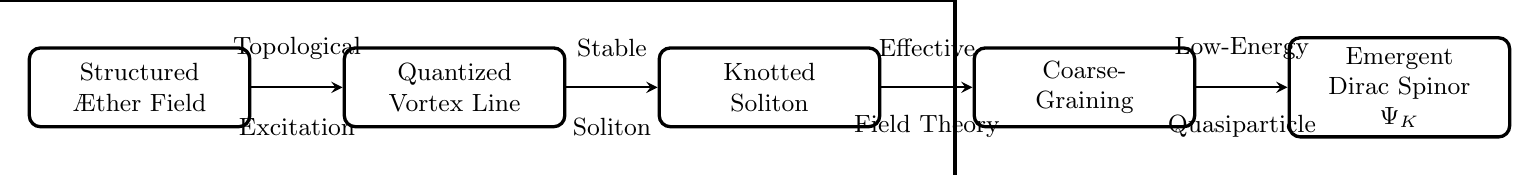
\begin{tikzpicture}[
            box/.style={rectangle, draw=black, very thick, rounded corners, minimum height=1cm, minimum width=2.8cm, align=center},
            arrow/.style={->, thick, >=stealth},
            every node/.style={font=\small}
        ]

% Nodes
            \node[box] (aether) at (0,0) {Structured \\ Æther Field};

            \node[box] (vortex) at (4,0) {Quantized \\ Vortex Line};

            \node[box] (knot) at (8,0) {Knotted \\ Soliton};

            \node[box] (coarse) at (12,0) {Coarse-\\Graining};

            \node[box] (dirac) at (16,0) {Emergent \\ Dirac Spinor \\ $\Psi_K$};

% Arrows
            \draw[arrow] (aether) -- (vortex);
            \draw[arrow] (vortex) -- (knot);
            \draw[arrow] (knot) -- (coarse);
            \draw[arrow] (coarse) -- (dirac);

% Labels
            \node at (2,0.5) {Topological};
            \node at (2,-0.5) {Excitation};

            \node at (6,0.5) {Stable};
            \node at (6,-0.5) {Soliton};

            \node at (10,0.5) {Effective};
            \node at (10,-0.5) {Field Theory};

            \node at (14,0.5) {Low-Energy};
            \node at (14,-0.5) {Quasiparticle};

        \end{tikzpicture}
        \caption{Schematic emergence of effective spinor fields in Vortex String Theory. Quantized vortices in a structured Æther give rise to topological solitons, which under coarse-graining behave like Dirac spinors in the effective theory.}
        \label{fig:emergent-spinors}
    \end{figure}


%========================================================================================
%   EMERGENT MASS FROM SOLITON ENERGY
%========================================================================================
    \section{Emergent Mass from Soliton Energy}

    For a static, stable knotted vortex configuration $K$, the rest energy $E_K$ defines the solitonic mass via $m_K^{(\mathrm{sol})} c^2 = E_K$. Guided by semiclassical analyses of knotted solitons \cite{Faddeev1997} and vortex energetics, we employ a phenomenological \emph{topological mass functional}
    \begin{equation}
        m_K^{(\mathrm{sol})}
        = \mathcal{M}_0 \; \Xi_K(m,n,s,k;\,\varphi)\,,
        \label{eq:mass-functional}
    \end{equation}
    where
    \begin{equation}
        \mathcal{M}_0 \equiv C_0 \left(\sum_i V_i\right) \rho_0 \frac{C_s^2}{c^2}
    \end{equation}
    sets the overall energy scale of the model. The function $\Xi_K$ is dimensionless and encodes topological information, including strand number ($m$), link number ($n$), tension/coherence indices ($s, k$), and golden-ratio suppression terms. The constant $\varphi$ enters through geometric identities associated with knotted-core packing.

    \subsection{Heuristic Derivation of the Mass Functional}

    To justify the structure of the topological mass functional in Eq.~\eqref{eq:mass-functional}, we consider a composite picture from fluid dynamics and knot soliton theory. A stable vortex configuration $K$ stores energy due to both the circulation of the core and its geometric topology.

    \vspace{0.5em}
    \paragraph{(1) Core Energy from Vortex Dynamics.}
    In classical fluid dynamics, the energy per unit length of a vortex line in an incompressible fluid is:
    \begin{equation}
        \frac{dE}{d\ell} \approx \frac{1}{2} \rho_0 \Gamma^2 \ln\left(\frac{R}{r_c}\right),
    \end{equation}
    where $\rho_0$ is the medium density, $\Gamma$ is the circulation, $r_c$ the core radius, and $R$ a characteristic external scale. The logarithmic term reflects the long-range kinetic energy.

    In our case, we replace $\Gamma \sim C_s\, r_c$ (with $C_s$ as a characteristic swirl velocity), and for a knotted vortex we integrate over the total arclength $\ell_K$:
    \begin{equation}
        E_K^{\text{core}} \sim \rho_0\, C_s^2\, \ell_K \ln\left(\frac{R}{r_c}\right).
    \end{equation}

    \vspace{0.5em}
    \paragraph{(2) Volume Correction and Dimensional Regularization.}
    The arclength $\ell_K$ scales with the number of strands and turns in the knot. To account for the full 3D core volume, we model the vortex as a tube of radius $r_c$ and write:
    \begin{equation}
        V_K = \sum_i \pi r_c^2\, \ell_i \ \Rightarrow\
        E_K^{\text{bulk}} \sim \rho_0\, C_s^2\, V_K.
    \end{equation}

    This term dominates in compact, tightly-wound knots and gives a leading energy proportional to mass density $\rho_0$ and internal velocity scale $C_s$.

    \vspace{0.5em}
    \paragraph{(3) Topological Suppression via Coherence.}
    To encode the knot structure, we introduce a dimensionless function $\Xi_K$, capturing:
    \begin{itemize}
        \item $m$: number of vortex strands.
        \item $n$: link crossings or writhes.
        \item $s$: coherence index (e.g., tension, alignment).
        \item $k$: golden suppression layer (Section~X).
    \end{itemize}

    The golden ratio enters as a scaling factor for internal coherence suppression:
    \begin{equation}
        \Xi_K(m,n,s,k;\varphi) = \frac{\mathcal{T}_{K}}{\varphi^{2k}},
    \end{equation}
    where $\mathcal{T}_K$ reflects geometric tangle energy, such as minimal ropelength or writhe number.

    \vspace{0.5em}
    \paragraph{(4) Putting It Together.}
    Combining all elements, the emergent soliton mass is:
    \begin{equation}
        m_K^{(\text{sol})} = \underbrace{C_0}_{\text{normalization}} \cdot
        \underbrace{\left( \sum_i V_i \right)}_{\text{core volume}} \cdot
        \underbrace{\rho_0\, \frac{C_s^2}{c^2}}_{\text{energy density scale}} \cdot
        \underbrace{\Xi_K(m,n,s,k;\varphi)}_{\text{topological weight}},
    \end{equation}
    as previously quoted in Eq.~\eqref{eq:mass-functional}. This gives a physically motivated, dimensionally consistent expression for mass in a vortex-string framework, suitable for benchmarking against known particle masses.


    \paragraph{Golden Ratio in Vortex Geometry.}
    The dimensionless mass factor $\Xi_K(m,n,s,k;\,\varphi)$ captures the topological and geometric contribution of the vortex core to total energy. The golden ratio $\varphi$ appears in this function through the hyperbolic layer index $k$, which reflects discrete energy quantization in confined, knotted vortex structures. Its role is physically motivated by several converging ideas:

    \begin{itemize}
        \item \textbf{Logarithmic Scaling:} In tightly packed flux tubes and vortex strands, optimal packing angles and self-avoiding curvature are governed by irrational constants, with the golden ratio emerging in minimal ropelength configurations \cite{Stasiak2009}.
        \item \textbf{Rapidity and Hyperbolic Geometry:} The definition of $\varphi$ via inverse hyperbolic sine allows a natural translation between spatial scaling (via $\varphi^{-k}$) and Lorentz-like rapidity suppression (via $\xi_g = \tfrac{3}{2}\ln\varphi$), linking the spatial configuration of the knot to its relativistic mass contribution.
        \item \textbf{Fractal Layering:} In multiscale soliton models, golden ratio scaling is associated with minimal energy growth across layers. The suppression term $\varphi^{-2k}$ represents a geometric decay in internal coherence of nested core layers.
    \end{itemize}

    The use of $\varphi$ is thus not arbitrary, but arises naturally from the geometric logic of vortex knots and the energy scaling of topologically constrained fields.


    \subsection{Calibration and Comparison}

    We fix $\mathcal{M}_0$ by calibrating against a single reference particle, typically the electron. Once set, the model's predictive content lies entirely in the topological ratios encoded by $\Xi_K$. This strategy avoids parameter overfitting and highlights the topological origin of mass ratios across leptons and hadrons.

    Predicted masses are then compared against experimental values \cite{PDG2024}, and model uncertainties are propagated by estimating fluctuations in vortex tension and coherence structure. Additional refinements could incorporate corrections due to vortex self-interaction energy or effective medium perturbations.


%========================================================================================
%   GAUGE STRUCTURE AND CHARGES
%========================================================================================
    \section{Gauge Structure and Charge Assignment}

    We treat the swirl gauge sector as an emergent non-Abelian group $G_{\!sw}$ generated by collective vorticity modes. At low energies, representations of $G_{\!sw}$ are mapped to Standard Model charges by knot invariants (writhe, twist, linking) and core-composition rules, in the spirit of topological preon models \cite{BilsonThompson2007}. Anomaly constraints are satisfied at the effective level by construction of the mapping; a full microscopic derivation is left for future work.

%========================================================================================
%   TOPOLOGY AND STABILITY
%========================================================================================
    \section{Topological Conservation and Stability}

    Knotted configurations are stabilized by conserved topological charges. In the gauge sector, $\mathcal{W}\tilde{\mathcal{W}}$ captures a Pontryagin density, while in the fluid/vorticity sector helicity invariants \cite{Moffatt1969,Arnold1998} and the fluxes of $\mathcal{H}=dB$ provide conserved integers. Experimental creation and persistence of knotted vortices in classical fluids \cite{Kleckner2013} motivate the use of similar invariants in the present medium.

%========================================================================================
%   CONCLUSION
%========================================================================================
    \section{Conclusion}

    We provided a consistent, covariant EFT for a vortex-string ontology of matter and interactions in a condensed vacuum with a preferred foliation. The action \eqref{eq:EFT} avoids nonrelativistic insertions, uses genuine topological densities, and cleanly separates condensate amplitude dynamics from emergent gauge structure. Masses enter as soliton energies via the topological functional \eqref{eq:mass-functional}. This formulation aligns with analogue-gravity intuition \cite{Barcelo2011,Volovik2003} and topological field theory \cite{Faddeev1997,Arnold1998}, and it is positioned for quantitative confrontation with data.

%========================================================================================
%   BIBLIOGRAPHY
%========================================================================================

    \printbibliography[title={References}]

    \appendix
    \section*{Appendix B: Emergent Gauge Fields from Vortex Coarse-Graining}
    \addcontentsline{toc}{section}{Appendix B: Emergent Gauge Fields from Vortex Coarse-Graining}
    \label{app:swirl-connection}


    The swirl gauge field \( \mathcal{A}_\mu^a \) appearing in the effective Lagrangian is interpreted as a coarse-grained representation of underlying vortex dynamics. This appendix outlines a heuristic derivation of such a connection from the mesoscopic averaging of vortex structures in a condensate.

    \subsection*{Mesoscopic Vorticity Fields}

    We begin with the microscopic vorticity 2-form in the fluid:
    \[
        \omega_{\mu\nu}(x) = \partial_\mu u_\nu - \partial_\nu u_\mu,
    \]
    where \( u^\mu \) is the unit timelike flow vector field. In a turbulent or knotted regime, this field exhibits complex structure on small scales (sub-knot size). We define a **mesoscopic average** over a coarse-graining scale \( \ell \) such that:
    \[
        \langle \omega_{\mu\nu}(x) \rangle \equiv \frac{1}{V_\ell} \int_{|x'-x|<\ell} \omega_{\mu\nu}(x')\, d^4x'.
    \]

    This averaging retains coherent structures larger than \( \ell \), such as vortex filaments and their interactions.

    \subsection*{Local Frames and Internal Indices}

    At each coarse-grained point, vortex lines may orient in different directions, twist, or braid. We define an orthonormal frame \( \{ e_a^\mu \} \) of preferred vortex orientations, satisfying:
    \[
        g_{\mu\nu} e^\mu_a e^\nu_b = \delta_{ab}, \qquad a=1,2,3.
    \]
    These local directions span a **fiber space** of possible swirl configurations. Variations in these directions under parallel transport induce a **connection field** \( \mathcal{A}_\mu^a \) analogous to a gauge field.

    \subsection*{Swirl Gauge Structure}

    We postulate that the collective rotation of vortex configurations defines a Lie algebra \( \mathfrak{g}_{sw} \) (e.g., \( \mathfrak{su}(2) \), \( \mathfrak{so}(3) \)). The gauge field then arises from the non-integrability of internal swirl alignment:
    \[
        \mathcal{A}_\mu = \mathcal{A}_\mu^a T^a,
    \]
    with \( T^a \in \mathfrak{g}_{sw} \). The curvature of this field encodes interactions:
    \[
        \mathcal{W}_{\mu\nu}^a = \partial_\mu \mathcal{A}_\nu^a - \partial_\nu \mathcal{A}_\mu^a + f^{abc} \mathcal{A}_\mu^b \mathcal{A}_\nu^c,
    \]
    where \( f^{abc} \) are the structure constants of the swirl group.

    \subsection*{Analogy with Liquid Crystals and Superfluids}

    This construction parallels well-known analogs:
    \begin{itemize}
        \item In superfluid \( ^3\mathrm{He} \), coarse-grained phase and spin textures define emergent gauge fields \cite{Volovik2009}.
        \item In nematic liquid crystals, distortions induce effective non-Abelian curvature tensors \cite{Lubensky2002}.
        \item In spinor BECs, internal spin degrees of freedom are associated with effective \( SU(2) \) gauge dynamics \cite{Ho1998}.
    \end{itemize}

    \subsection*{Implications and Effective Dynamics}

    The swirl gauge field \( \mathcal{A}_\mu^a \) couples to the spinor excitations \( \Psi_K \) via the covariant derivative:
    \[
        D_\mu = \partial_\mu + i g_{sw}\, \mathcal{A}_\mu^a T^a.
    \]
    This term in the effective action allows for **topological conservation**, helicity transport, and vortex-based gauge mediation effects.

    Future work should aim to derive the effective Yang–Mills term from vortex dynamics, using variational coarse-graining techniques or renormalization group flow.


\end{document}